% !TEX root = ../main.tex
\chapter{Results and Discussion}\label{ch:results}
This chapter will look into the results we gained after running the analysis across all opponents.
As of writing this section there are strategies missing from the analysis due to run times.
Details of the distribution of the results and basic output from the computation are given in section~\ref{sec:descriptive_data}.

The analysis performed in this chapter contains data for opponents listed in Appendix~\ref{apndx:opponents}.
Opponents without data due to being incomplete are all the (LRT) strategies listed.
As these become available they will be added to the analysis.

\section{Descriptive Data}\label{sec:descriptive_data}
loading, cleaning data, description data

\begin{figure}[ht]
    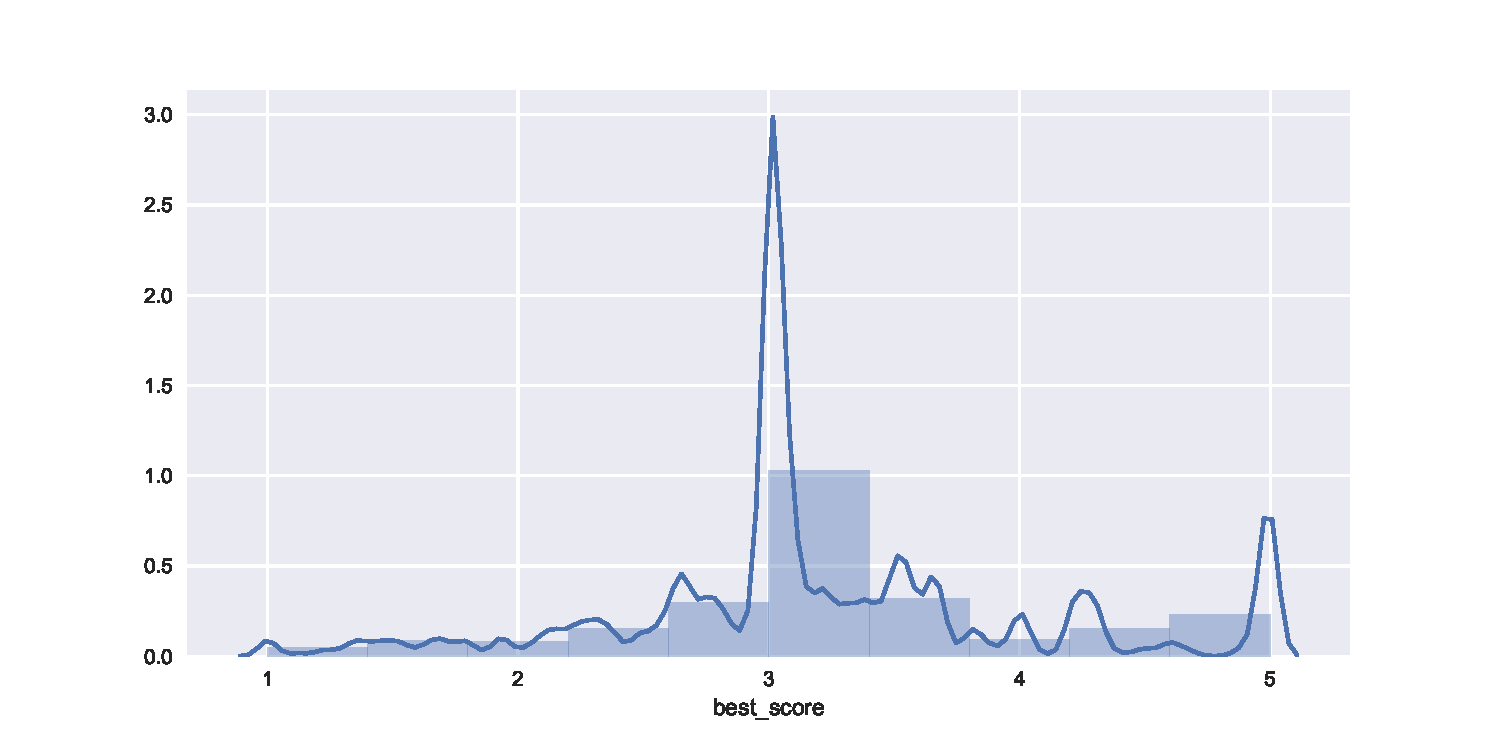
\includegraphics[width=0.7\textwidth, center]{./img/descriptive/best_score_hist.pdf}
    \caption{A histogram showing the distribution of best scores with overlaid kernel density estimate}\label{fig:best_score_hist}
\end{figure}

\section{Solution Distance Matrices}
The first avenue of analysis, after constructing descriptive data, was to look at the relationship strategies have with each other.
A distance matrix shows how much an opponent differs from every other, if 2 sequences are similar with respect to the distance function then they will score lower than 2 sequences that are more distinct.
Certain distance functions have been selected because of their connotations.

In each matrix we order the sequences by score; $S_{O_0}\ge S_{O_1} \ge \ldots \ge S_{O_n}$, but we will shorten $S_{O_i}$ to $S_{i}$ for simplicity.
The solution sequence for the $i$th opponent, $S_i$ vs the solution sequence for the $j$th, $S_j$ is scored using our distance function, for example $d(S_0,S_n)$ is the distance between the best and worst scoring sequences respectively.
The Matrix itself will be symmetric, so looking across rows vs columns tends to make more logical sense; the top rows are the highest scoring opponents, and the lower rows the worse scorers.

\paragraph{Hamming Distance}
$$d(S_i,S_j) = S_i \cdot S_j^T \text{ or } 1-\frac{\sum^n_{i,j=0}\delta_{ij}}{n}\text{ where } \delta_{ij} = \begin{cases} 
    1 & i=j \\
    0 & i\ne j 
\end{cases} $$

The Hamming Distance represents the count of the elements that differ in any two sequences. 
A Hamming Distance will thus correspond to the number of places we have to play different moves against opponents to get out best score. 
Figure~\ref{fig:dist_ham} shows the matrix generated by the code in Figure~\ref{apcode:dist_matrix.py}.

By observing the graph row by row, we can build an idea of how similar each sequence is to the range of others.
the top section of the plot shows the best scoring opponents vs themselves on the left and the worse scoring opponents on the right. 
At the very top  left there is lots of darker rows, suggesting that there are lots of very similar or dissimilar solutions at the high end of the score level, as we move to the right we have many slightly similar opponents then on the far right lots of very different sequences.
This is shown again as we move to the bottom of the diagram.
The large blocks or red covering the bottom  100 or so rows show that the lowest scoring opponents have very different sequences to the higher scorers, but as a group on the bottom right they're quite similar.

The result of an average score means that we can estimate the distribution of move combinations because we know, if we are the first player: $(C,C)=3$, $(C,D)=0$, $(D,C)=5$, $(D,D)=1$.
Thus if we assume scoring in the midrange ($3$ ish) means mostly cooperating or a combination of $(C,D)$ and $(D,C)$ whereas at the high and low ends its more likely to be defecting.
Thus if we assume scoring in the midrange ($3$ ish) means mostly cooperating or a combination of $(C,D)$ and $(D,C)$ whereas at the high and low ends its more likely to be defecting.
Looking at the high va low and low vs high scoring sections of the graph this hypothesis isn't supported, we would expect them to have $d(S_i,S_j)\approx 0$, whereas were seeing a mix of distances. 
Section~\ref{sec:solutionGroups} looks at patterns of move density vs best score.

\paragraph{Cosine Distance}
$$ d(S_i,S_j) = cos(\theta) = \frac{{S_i} \cdot {S_j}}{|| {S_i} || \; || {S_j} ||} $$
The cosine of two vectors constructed by using the dot product formula as shown above.
% Figure~\ref{fig:cosine} shows an interpretation of this in 2 dimensions
In our interpretation each dimension represents a sequence element so we are working in $\mathbb{R}^{200}$ with every value taking a $C:1$ a $D:0$.
% \begin{figure}[h]
%     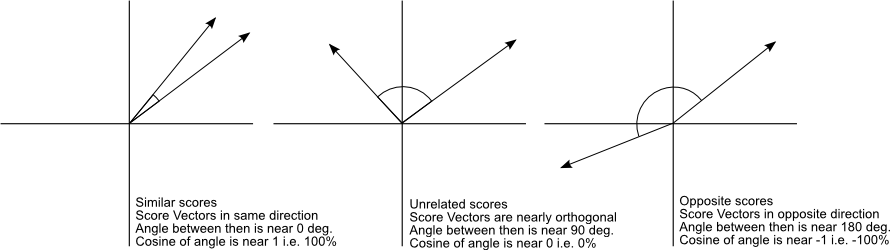
\includegraphics[width=1.0\textwidth, center]{./img/examples/cosinesimilarity.png}
%     \caption{An Example of 2d cosine similarity~\cite{Perone2013blog}}\label{fig:cosine}
% \end{figure}
Figure~\ref{fig:dist_cos} shows the distance matrix generated from the data files using code in Figure~\ref{apcode:dist_matrix.py}

The Matrix for Cosine and Hamming are almost exactly similar, the only difference being the value of the distance between sequences.
This is due to the two measures being similar in their relationship of space~\cite{choi2010survey}.
We can conclude that there is no extra information shown in this diagram.
\begin{figure}[ht]
    \centering
    \begin{minipage}{0.48\textwidth}
        \centering
        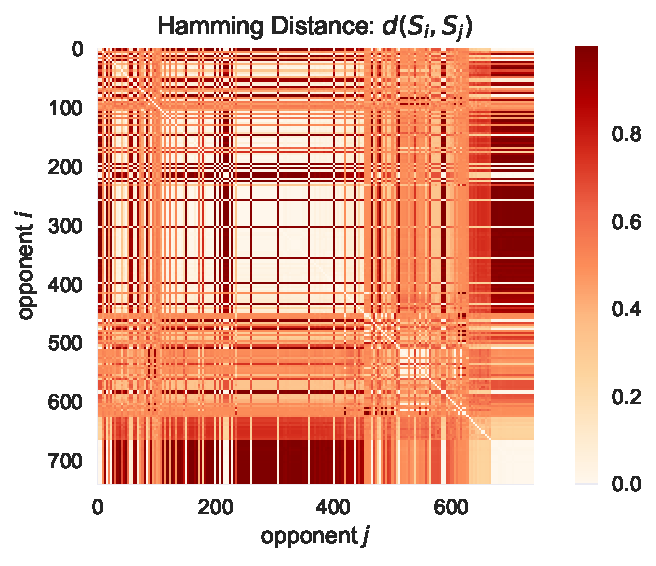
\includegraphics[width=1.0\textwidth, center]{./img/dist_matrix/dist_ham.pdf}
        \caption{Distance Matrix for Hamming Distance}\label{fig:dist_ham}
    \end{minipage}\hfill
    \begin{minipage}{0.48\textwidth}
        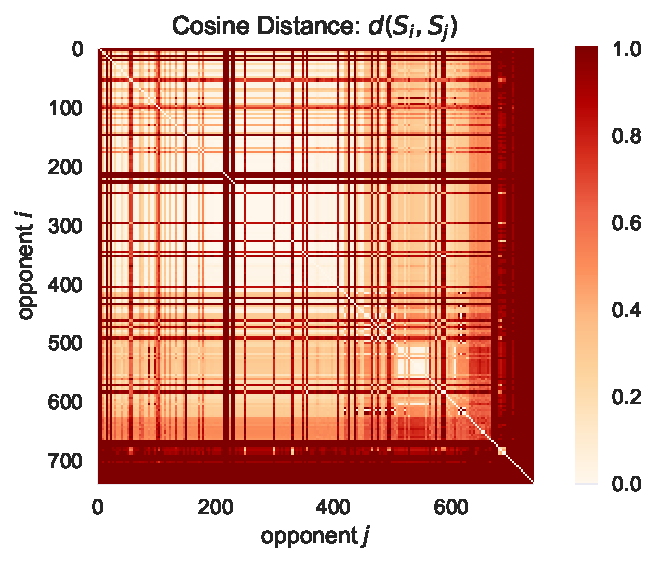
\includegraphics[width=1.0\textwidth]{./img/dist_matrix/dist_cos.pdf} 
        \caption{Distance Matrix for Cosine Distance}\label{fig:dist_cos}
    \end{minipage}
\end{figure}

\section{Solution Groups}\label{sec:solutionGroups}
If we want to group opponents together, the most obvious way is to look at which opponents have have the same best score sequence.
Appendix section~\ref{apndx:solutionGroups} has full details, but figure~\ref{fig:sequence_scatter} shows a plot of the trends. 
We can observe that there are lots of sequences with solutions that dont contain many blocks ($\le 25$)
\begin{figure}[ht]
    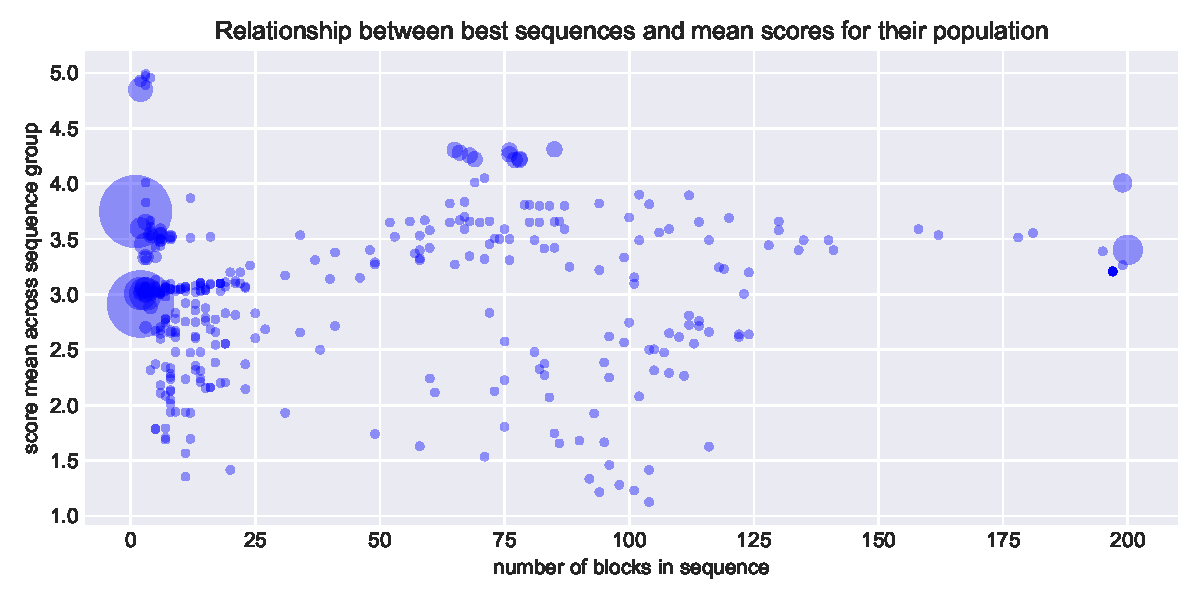
\includegraphics[width=0.7\textwidth, center]{./img/descriptive/sequence_scatter.pdf}
    \caption{Trends for opponents grouped by their best sequence}\label{fig:sequence_scatter}
\end{figure}

\begin{figure}[ht]
    \centering
    \begin{minipage}{0.48\textwidth}
        \centering
        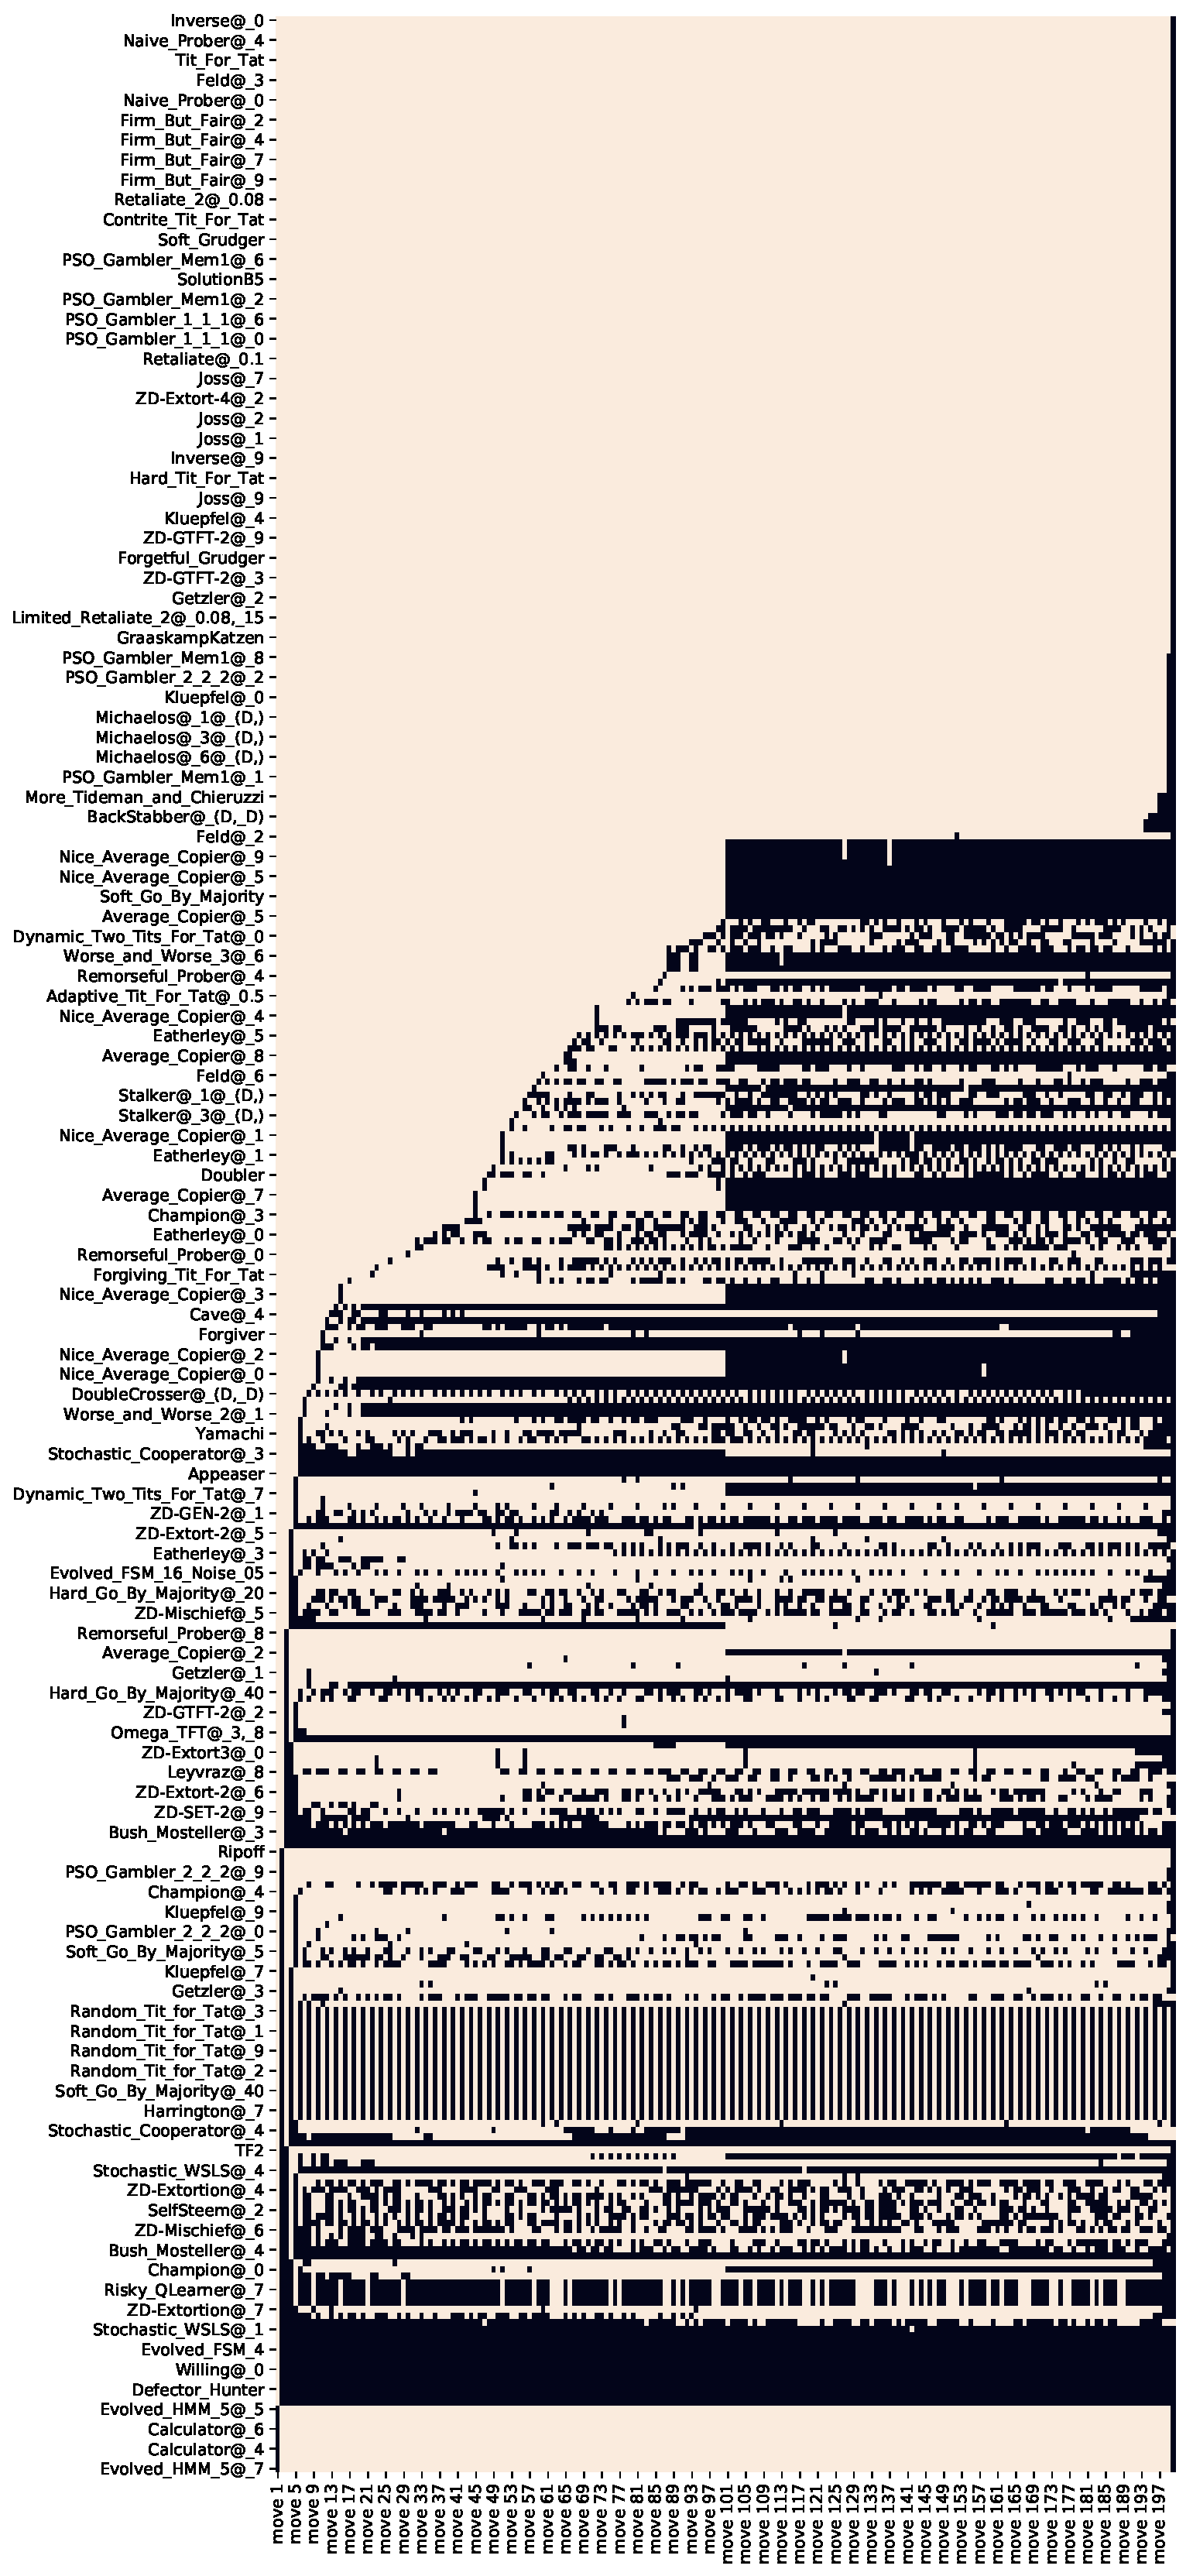
\includegraphics[width=1.0\textwidth, center]{./img/descriptive/sequence_plot_alphabetical_pt1.pdf}
    \end{minipage}\hfill
    \begin{minipage}{0.48\textwidth}
        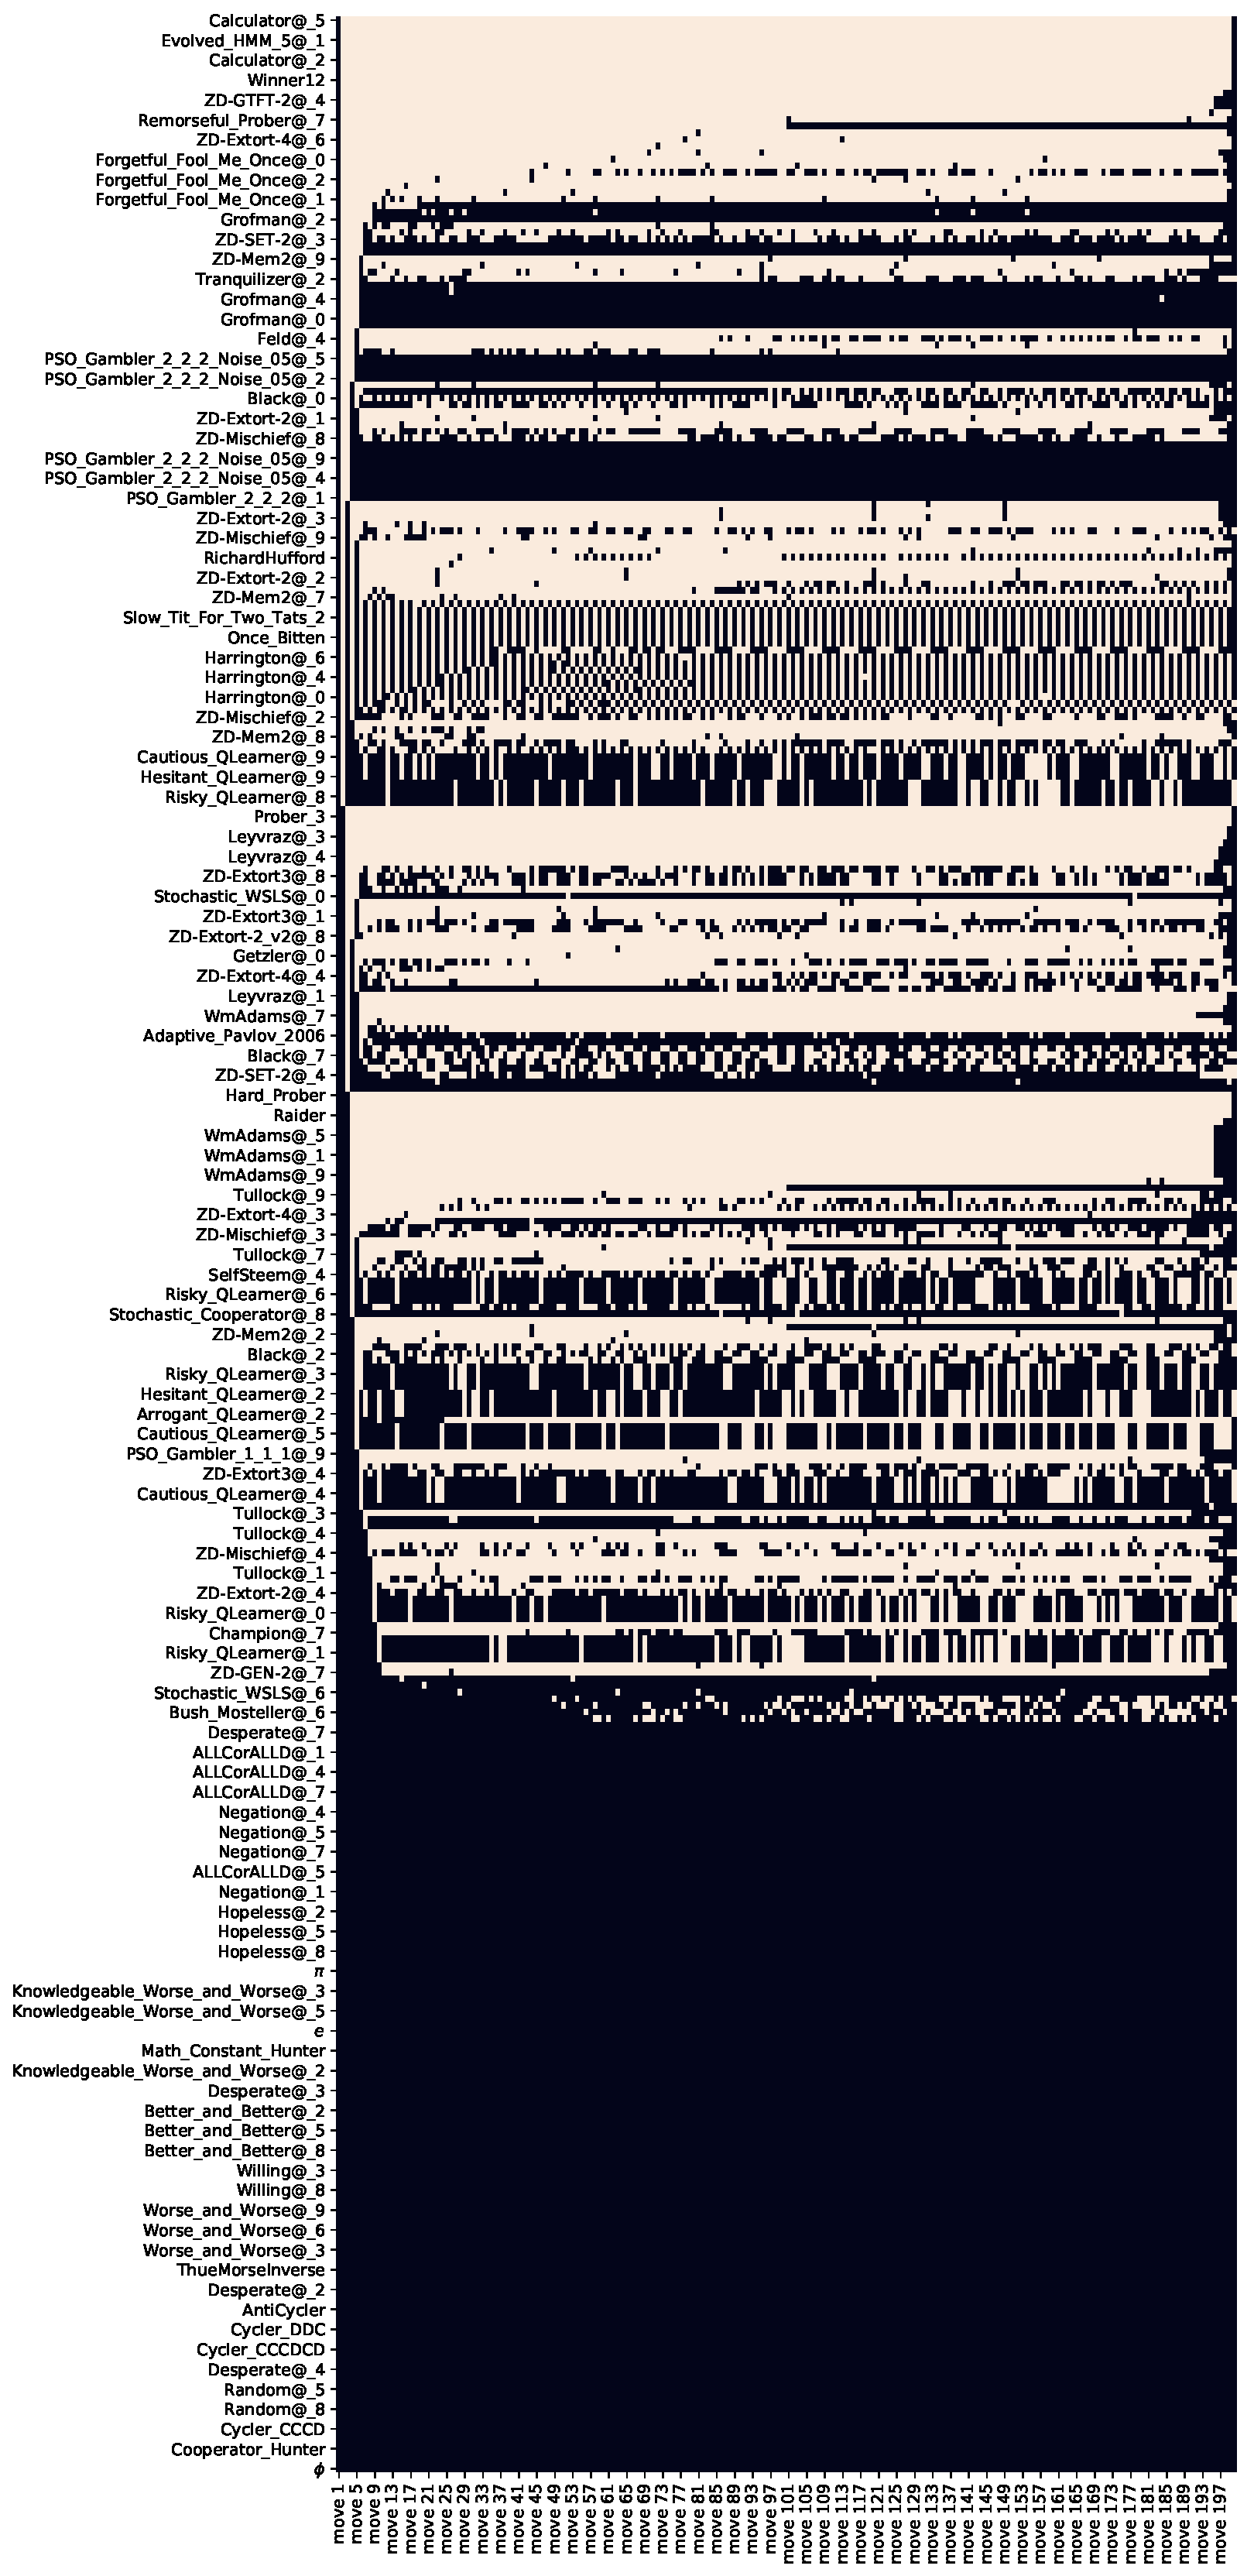
\includegraphics[width=1.0\textwidth, center]{./img/descriptive/sequence_plot_alphabetical_pt2.pdf}
    \end{minipage}
    \caption{Sequence Diagram, sorted by move in turns}\label{fig:sequence_plot_alphabetical}
\end{figure}

\section{Scoring Groups}

\begin{figure}[ht]
    \centering
    \begin{minipage}{0.48\textwidth}
        \centering
        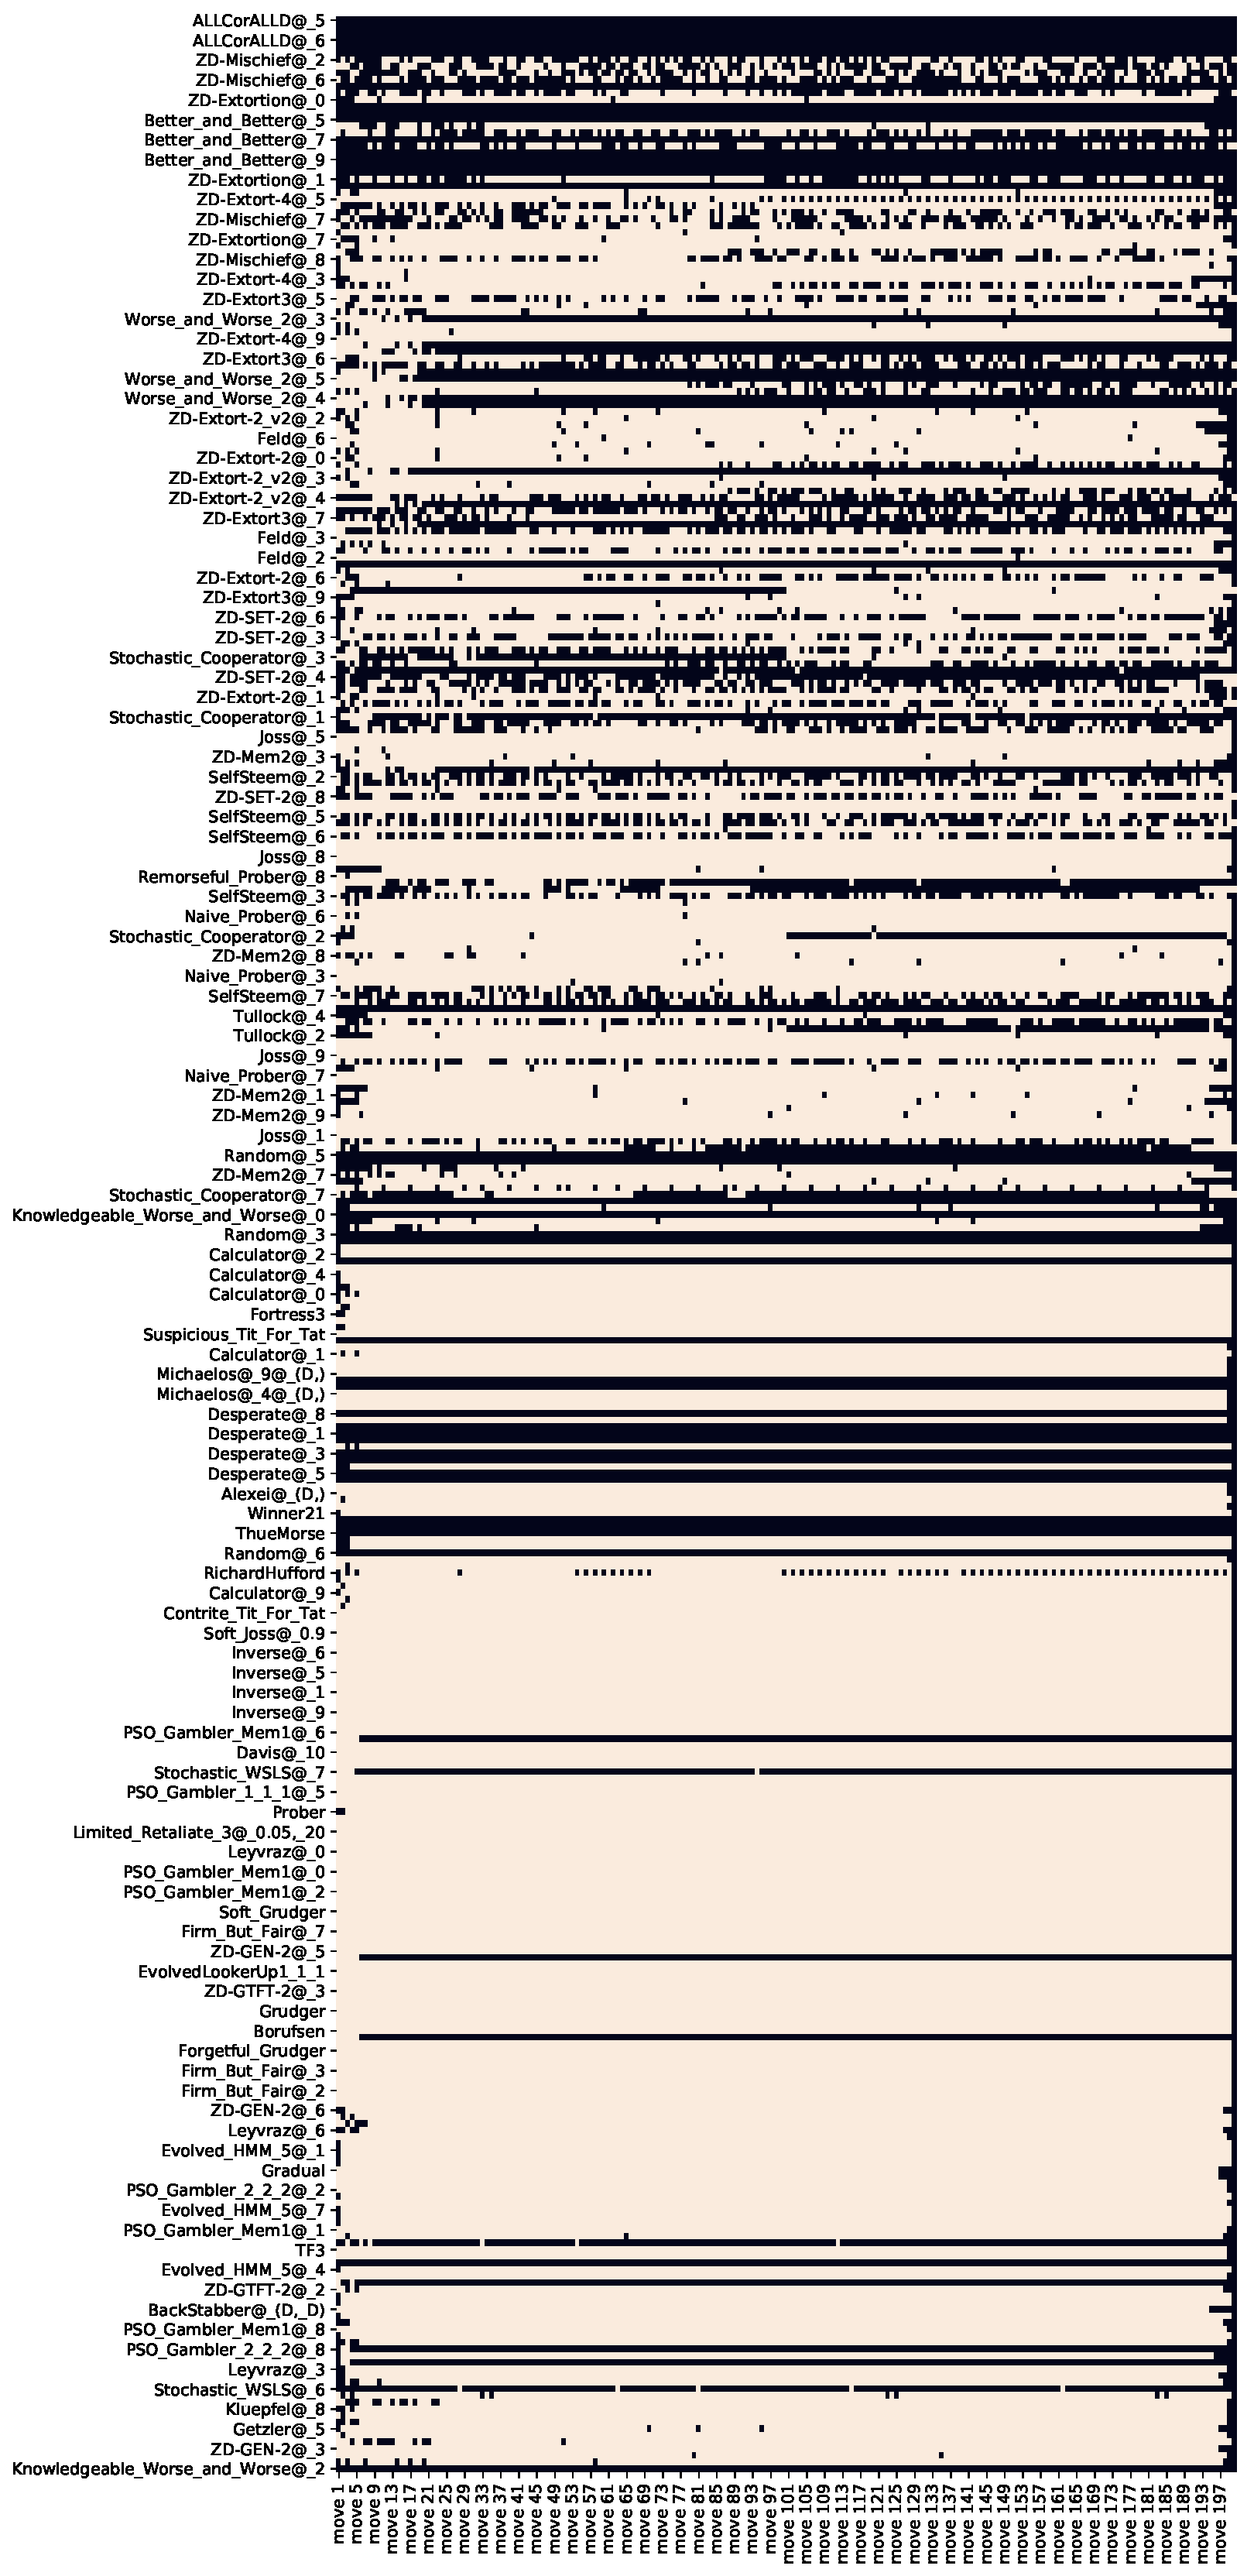
\includegraphics[width=1.0\textwidth, center]{./img/descriptive/sequence_plot_score_pt1.pdf}
    \end{minipage}\hfill
    \begin{minipage}{0.48\textwidth}
        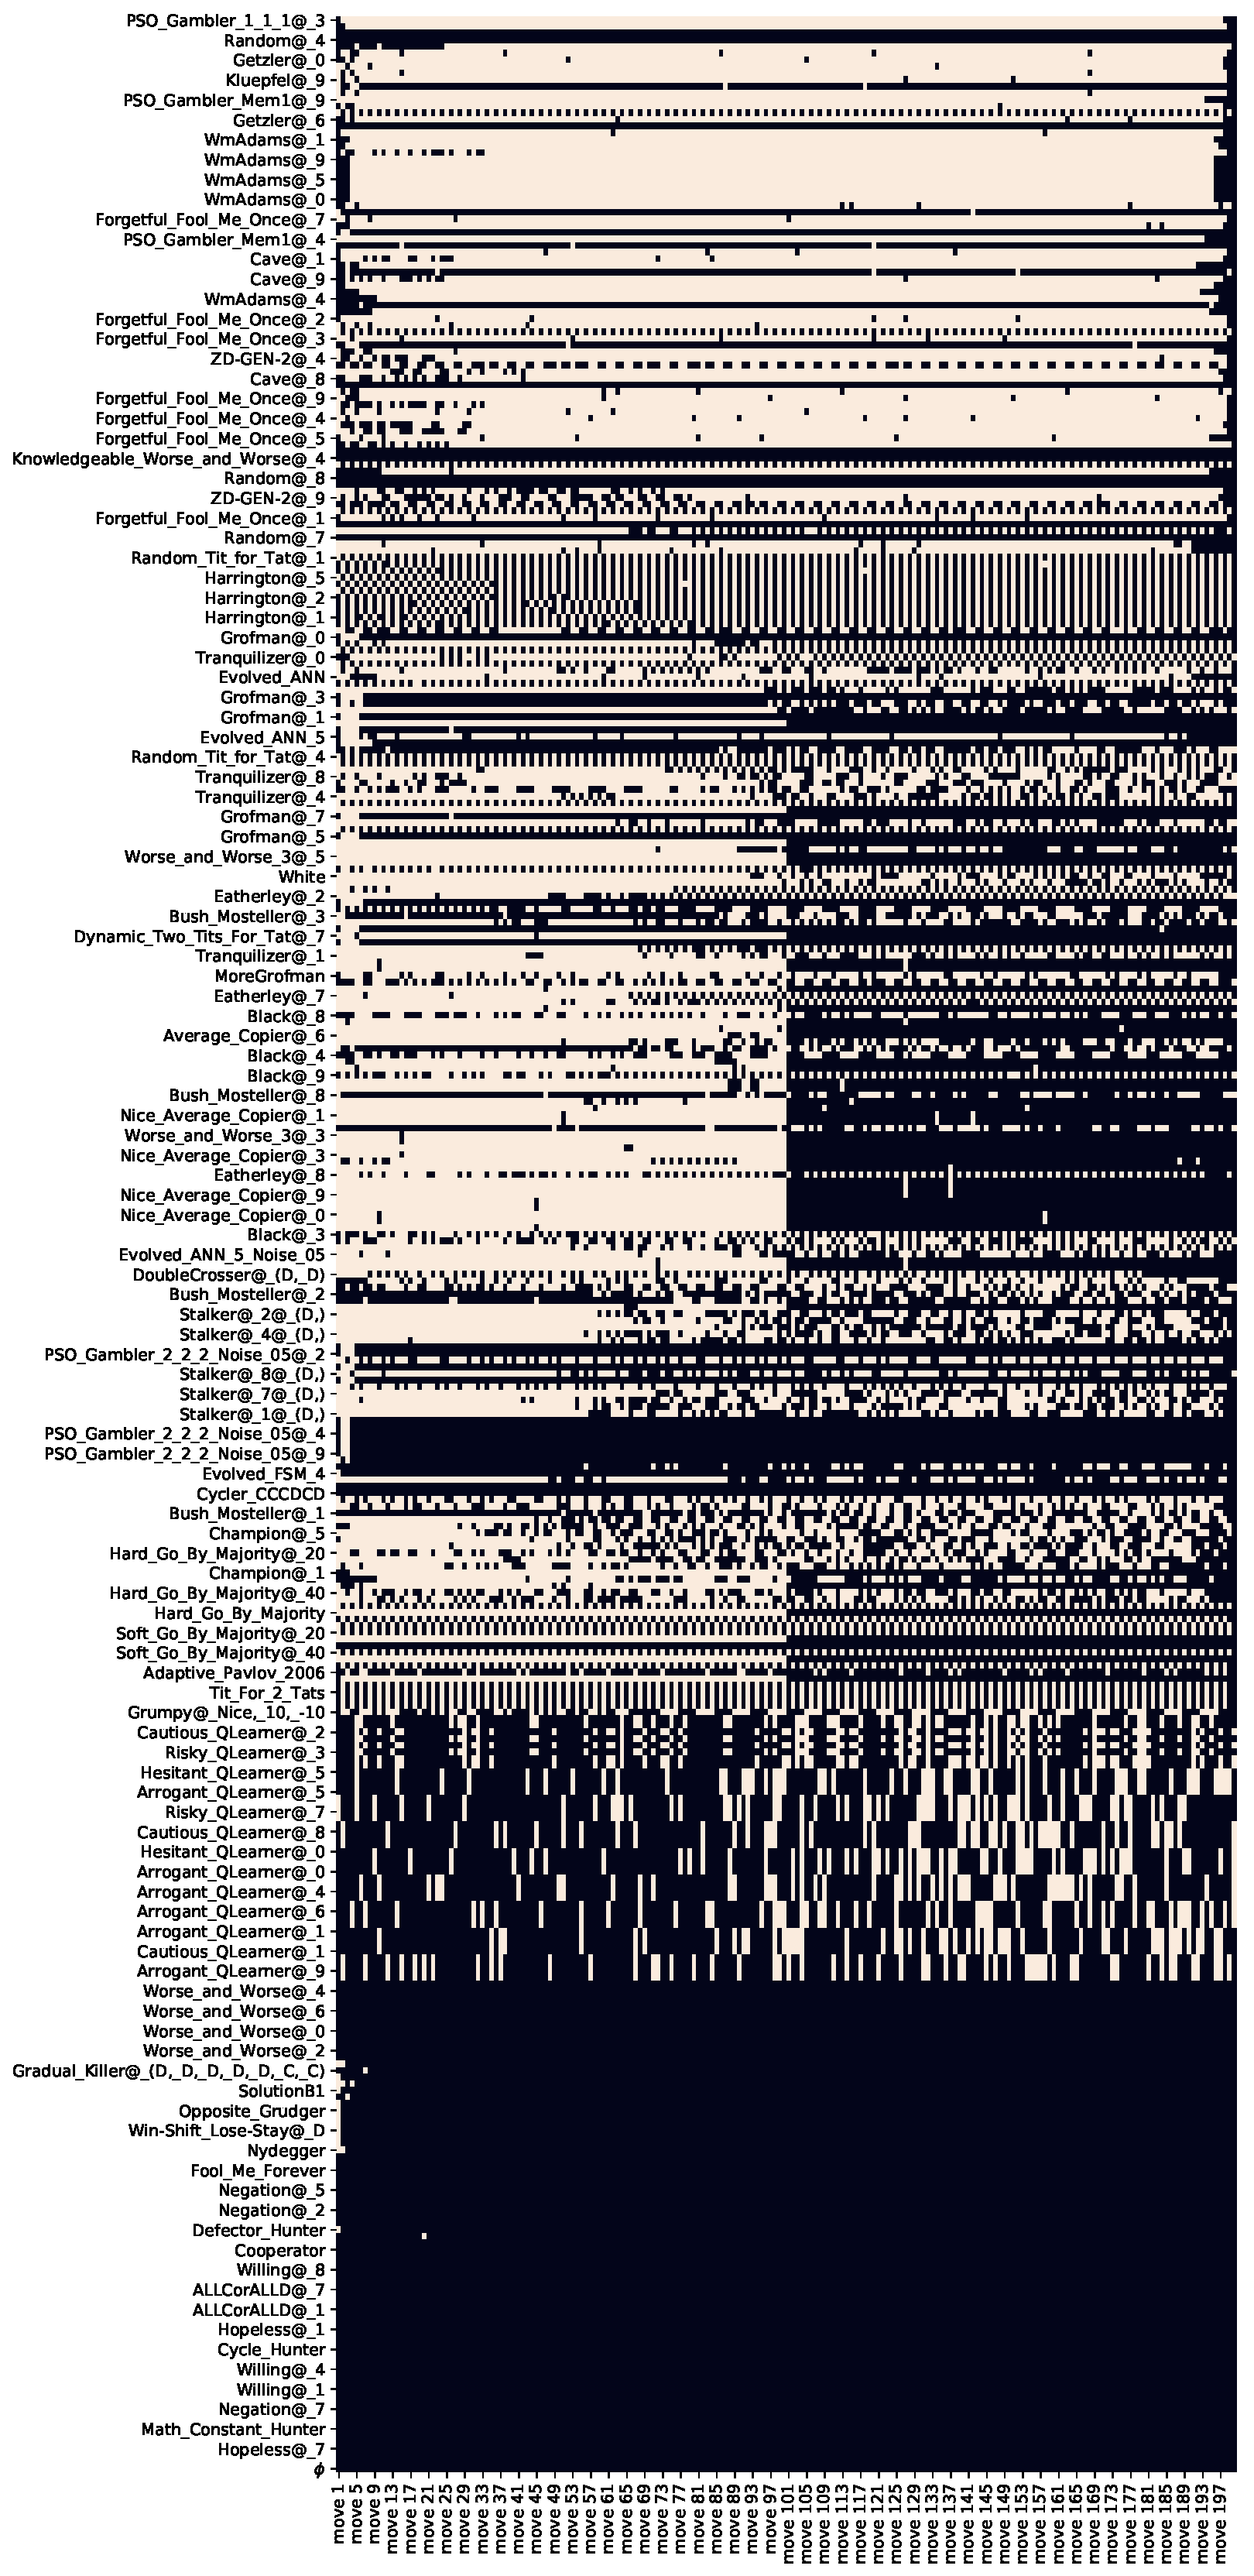
\includegraphics[width=1.0\textwidth, center]{./img/descriptive/sequence_plot_score_pt2.pdf}
    \end{minipage}
    \caption{Sequence Diagram, sorted by score}\label{fig:sequence_plot_score}
\end{figure}

\section{Clustering Analysis}
Here we will look at ways of grouping opponents and what that means for potential scoring outcomes.
\subsection{K Means clustering}\label{ssec:k_means}


\subsection{Classification Trees}
Classification trees are a way of looking at reducing the variance of a parameter through attributes of observed instances. 
In our case were looking at reducing the variance of the score by looking at which turns tend to cause the largest disparity in score.
To do this we look at reducing the Mean Absolute Error of the scores, which is, in effect reducing the $L1$ loss of the scores.

$$MAE = \frac{1}{n}\sum_{i=0}^n |x_i-y_i|$$

\begin{sidewaysfigure}
    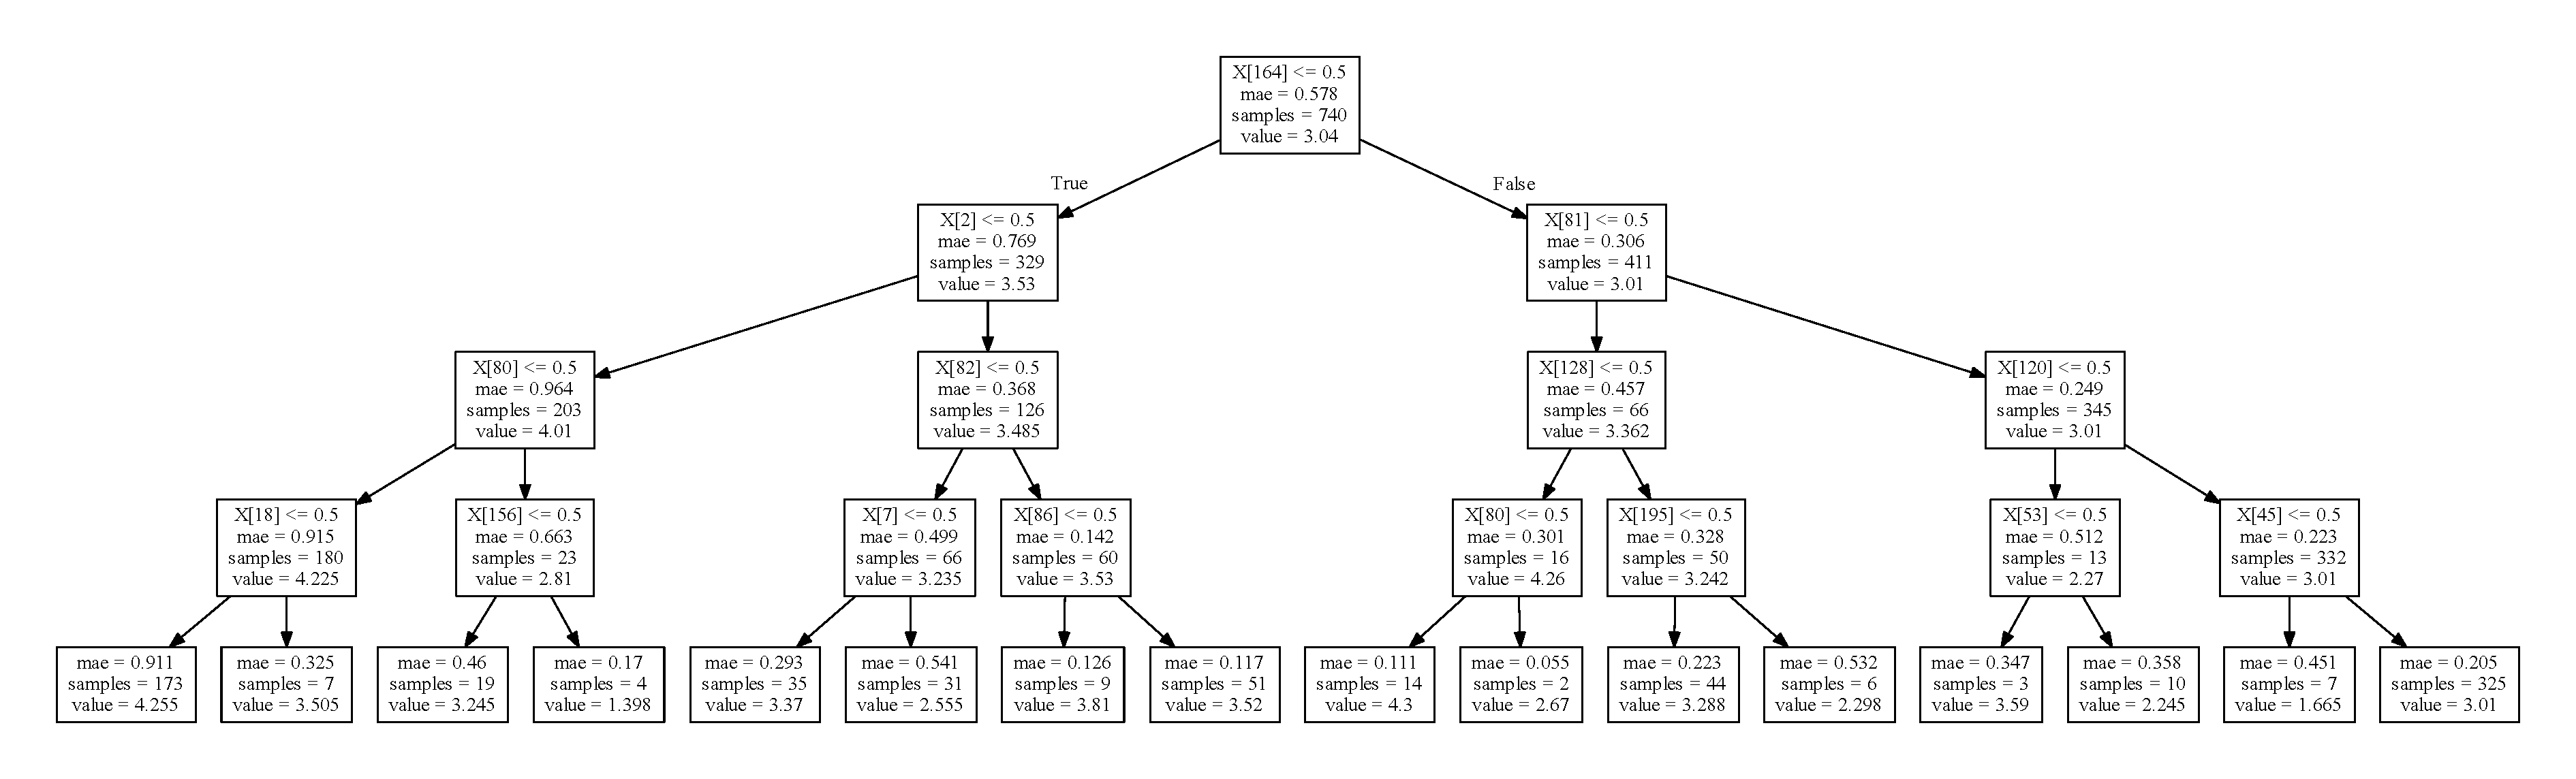
\includegraphics[width=1.0\textwidth, center]{./img/descriptive/reg_tree.pdf}
    \centering
    \caption{A regression tree showing which moves introduce the largest absolute error in the best score. If $X[i]>=0.5$ is true, it means move $i$ is a Cooperation move. $(C:1,D:0)$}\label{fig:reg_tree}
\end{sidewaysfigure}


\section{Conclusion}